\documentclass[12pt]{article}
\usepackage[hidelinks]{hyperref}    
\usepackage[all]{hypcap}
\usepackage{graphicx}
\usepackage{amsmath}
\graphicspath{{../../_images/}}
\author{Andrea Malvezzi}
\title{\textbf{Logica per l'informatica~-~Lezione 0}}
\date{20 Settembre, 2024}
\begin{document}
\maketitle
\pagebreak
\tableofcontents
\pagebreak
\section{Cos'è la logica proposizionale}
La logica proposizionale è una logica meno espressiva di quella del prim'ordine e si usa per studiare solamente \textbf{proposizioni} (quindi niente numeri etc $dots$).\\
In questo tipo di logica si passa da un ragionamento ad una formalizzazione in linguaggio logico e quindi risulta fondamentale comprendere e tradurre bene la frase.
\section{Sintassi della logica proposizionale}
Qui si usano meno simboli rispetto alla logica del prim'ordine e si procede mediante alberi di deduzione naturali.\\
Ecco la simbologia completa:
\begin{itemize}
    \item Falso $\rightarrow \bot$ (bottom);
    \item Vero $\rightarrow \top$ (top);
    \item Si possono usare variabili indicate con lettere dell'alfabeto $A, B, C, \dots$;
    \item $A$ negato $\rightarrow \not A$;
    \item $A$ e $B \rightarrow A \wedge B$;
    \item $A$ oppure $B \rightarrow A \vee B$;
    \item se $A$ allora $B \rightarrow A \Rightarrow B$, se si ha $B$ allora SICURAMENTE si ha $A$, ma se si ha $A$ non è detto che si abbia anche $B$.
\end{itemize}
\pagebreak
\section{Gli alberi di deduzione naturale}
I logicia scrivono gli alberi dal basso verso l'alto ma li possono leggere sia dall'alto verso il basso (come gli informatici) e sia dal basso verso l'alto.
\subsection{Esempio pratico}
Avendo $B,D \wedge A \vdash A \wedge (B \Rightarrow C) \Rightarrow C$, allora:
\begin{itemize}
    \item la parte antecedente $\vdash$ si dice \textbf{Gamma} ($\Gamma$) e contiene le \textbf{ipotesi globali};
    \item la parte dopo $\vdash$ si dice \textbf{radice}, indicata con $F$, ed equivale a ciò che vogliamo effettivamente dimostrare;
    \item ad ogni linea orizzontale usata per dividere i vari layer di un albero equivale un passaggio, ovvero una regola degli operatori elencati in precedenza, come l'introduzione dell'and e simili;
    \item il simbolo $\vdash$ indica una derivazione: da Gamma derivo la radice, ovvero, in linguaggio logico: $\Gamma \vdash F$.
\end{itemize}
E l'albero della formula presa come esempio sarebbe:
\begin{figure}[!htb]
    \centering
    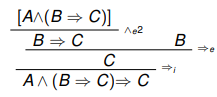
\includegraphics[width=.9\linewidth,height=.40\textheight,keepaspectratio]{logica_proposizionale/introduzione/albero_deduzione.png} % essenzialmente resiza l'immagine
    \begin{center}
        \caption{\label{fig:}Esempio di albero di deduzione naturale.}
    \end{center}
\end{figure}
\section{Le regole}
Nella figura seguente $F_n$ sono dette \textbf{premesse} della regola che si vuole applicare, mentre $F$ si dice \textbf{conclusione} della regola.
\begin{figure}[!htb]
    \centering
    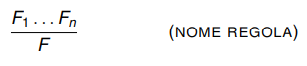
\includegraphics[width=.9\linewidth,height=.40\textheight,keepaspectratio]{brutta/regole_albero.png} % essenzialmente resiza l'immagine
    \begin{center}
        \caption{\label{fig:regole_albero}Esempio di albero con n regole e una conclusione (ovviamente).} % label fuori da caption spesso non va, mettilo dentro
    \end{center}
\end{figure}\\
Una regola senza premesse si dice assioma (ma è diverso da quelli della logica del primo ordine).
\subsection{Invertibilità di una regola}
Una regola si dice invertibile quando la sua conclusione implica le ipotesi, ovvero quando c'è \textbf{coimplicazione} tra conclusione e premesse.\\
Questa proprietà risulta utile in quanto permette di ragionare in entrambi i versi durante una dimostrazione.\\
Applicare una regola invertibile non è quasi mai errato in quanto si possono sempre utilizzare, proprietà di cui le regole non-invertibili non godono.
\section{AND}
\subsection{Regola di introduzione}
La regola di introduzione dell'\textit{and} si indica con $\wedge_i$ e consiste in:
\begin{equation}
    \dfrac{F_1 \text{ } F_2}{F_1 \wedge F_2} \label{rule:and_intro}
\end{equation}
Lettura bottom-up (dalle premesse alla radice): se $F_1$ e $F_2$ allora $F_1 \wedge F_2$.\\
Lettura top-down (dalla radice alle premesse): per dimostrare $F_1 \wedge F_2$ allora devo dimostrare sia $F_1$ che $F_2$.\\
\textbf{N.B.:} spesso le regole che "suonano bene" in italiano sono invertibili.
\subsection{Regola di eliminazione}
La regola di eliminazione dell'\textit{and} si indica con $\wedge_e$ e consiste in:
\begin{figure}[!htb]
    \centering
    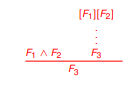
\includegraphics[width=.9\linewidth,height=.40\textheight,keepaspectratio]{logica_proposizionale/introduzione/eliminazione_and.png} % essenzialmente resiza l'immagine
    \begin{center}
        \caption{\label{fig:eliminazione_and}Regola di eliminazione dell'and.} % label fuori da caption spesso non va, mettilo dentro
    \end{center}
\end{figure}\\
Lettura bottom-up: se $F_1 \wedge F_2$ e se ipotizzando $F_1$ e $F_2$ concludo $F_3$, allora $F_3$.\\
Lettura top-down: per dimostrare $F_3$ data l'ipotesi $F_1 \wedge F_2$ è sufficiente dimostrare $F_3$ sotto le ipotesi $F_1$ e $F_2$.\\
Questa regola splitta in due rami come l'introduzione, ma mentre in essa si ha spesso una premessa verificata per altre ipotesi, qui si deve procedere a dimostrare entrambe e in $F_3$ occorre usare anche le ipotesi $F_1$ e $F_2$.
\subsubsection{Non-invertibile}
\textbf{N.B.:} la regola NON è \textbf{SEMPRE} invertibile, in quanto supponendo $F_1$ o $F_2 = \bot$ e $F_3 = \top$ si ha $\top \not\vdash \bot \wedge \bot$.
Tuttavia, diviene invertibile nei casi in cui si assume $F_1 \wedge F_2 = \top$, in quanto:
\[F_3 \vdash F_1 \Rightarrow F_2 \Rightarrow F_3\]
\subsection{Regole alternative di eliminazione}
Ci sono altre due regole alternative di eliminazione (entrambe non invertibili in alcun caso):
\begin{gather}
    \dfrac{F_1 \wedge F_2}{F_1}, (\wedge_{e_1}) \label{rule:and_elim_1}\\
    \dfrac{F_1 \wedge F_2}{F_2}, (\wedge_{e_2}) \label{rule:and_elim_2}
\end{gather}
\subsection{Riassunto regole dell'AND}
La regola di eliminazione risulta utile per spezzare un'ipotesi congiunta (del tipo $A \wedge B$) nelle sue sottoparti. Questo si può fare anche per le ipotesi globali (o \textit{iniziali}), per frammentarle e poterle poi usare nell'intero scope del ramo su cui si sta operando.\\
La regola di introduzione risulta utile per semplificare la conclusione della regola nelle componenti che la compongono.
\pagebreak
\section{OR}
\subsection{Regole di introduzione}
Le regole di introduzione dell'\textit{or} si indicano con $\vee_{i_1}$ e $\vee_{i_2}$ e consistono in:
\begin{gather}
    \dfrac{F_1}{F_1 \vee F_2},\vee_{i_1}  \label{rule:or_intro_1}\\
    \dfrac{F_2}{F_1 \vee F_2},\vee_{i_2}  \label{rule:or_intro_2}
\end{gather}
Non sono invertibili e dato che non permettono di splittare, si opta prima per la regola di eliminazione, ovvero $\dots$
\subsection{Regola di eliminazione}
La regola di eliminazione dell'\textit{or} si indica con $\vee_e$ e consiste in:
\begin{figure}[!htb]
    \centering
    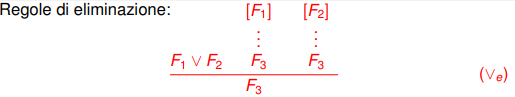
\includegraphics[width=.9\linewidth,height=.40\textheight,keepaspectratio]{logica_proposizionale/introduzione/eliminazione_or.png} % essenzialmente resiza l'immagine
    \begin{center}
        \caption{\label{fig:eliminazione_or}Regola di eliminazione dell'or.} % label fuori da caption spesso non va, mettilo dentro
    \end{center}
\end{figure}\\
La regola non è \textbf{sempre} invertibile: $F_3 = \top$ e $F_1 = F_2 = \bot$.\\
Tuttavia lo diventa quando posso dimostrare $F_1 \vee F_2$.
\pagebreak
\section{Armonia nell'AND e nell'OR}
Ma come mai le formule di eliminazione sono scritte in questo modo?\\
Partiamo dall'AND: qui abbiamo una sola regola di introduzione, quindi una congiunzione si può introdurre solamente con una certa scrittura (vedi (\ref{rule:and_intro})). Ciò significa che, una volta giunti ad avere una congiunzione, allora si avranno sicuramente le sue due ipotesi iniziali ($F_1$ e $F_2$). Quindi avendo quelle due ipotesi iniziali si può affermare con certezza che si avrà anche $F_3$ (vedi (\ref{fig:eliminazione_and})):
\begin{figure}[!htb]
    \centering
    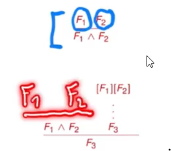
\includegraphics[width=.9\linewidth,height=.40\textheight,keepaspectratio]{logica_proposizionale/introduzione/armonia_and.PNG} % essenzialmente resiza l'immagine
    \begin{center}
        \caption{\label{fig:armonia_and}Dimostrazione dell'armonia dell'AND.} % label fuori da caption spesso non va, mettilo dentro
    \end{center}
\end{figure}\\
La stessa cosa vale per l'OR: qui si hanno due regole di eliminazione e per introdurre una disgiunzione serve o una ipotesi o l'altra, quindi sicuramente potrò dedurre $F_3$ a partire o da $F_2$ o da $F_1$.
\pagebreak
\section{BOTTOM}
Il bottom ($\bot$) indica qualcosa di sempre falso e perciò di non dimostrabile direttamente, ma bensì solo attraverso l'eliminazione di ipotesi.\\
Non avrà quindi una regola di introduzione (diretta), ma solamente una di eliminazione $\dots$
\subsection{Regola di eliminazione}
La regola di eliminazione del \textit{bottom} si indica con $\bot_e$ e consiste in:
\begin{equation}
    \dfrac{\bot}{F} \label{rule:bot_elim}
\end{equation}
A causa dell'armonia possiamo affermare che, data la mancanza di regole di introduzione, serviranno zero casi (premesse) per eliminare il bottom e dimostrare qualunque cosa.
\subsubsection{Non-Invertibilità}
Questa regola non è invertibile ma si usa bensì quando si \textbf{intuisce all'avanti (guardando avanti)} che qualcosa potrebbe essere sempre falso.
\section{TOP}
Il TOP ha una regola di introduzione (ed è quindi dimostrabile), ma non ha bisogno di premesse (si dice perciò \textbf{assioma}).
\subsection{Regola di introduzione}
La regola di introduzione si indica con $\top_i$ e consiste in:
\begin{equation}
    \dfrac{}{\top}  \label{rule:top_intro}
\end{equation}
\pagebreak
\section{IMPLICAZIONE}
\subsection{Regola di introduzione}
La regola di introduzione dell'implicazione si indica con $\Rightarrow_i$ e consiste in:
\begin{figure}[!htb]
    \centering
    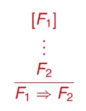
\includegraphics[width=.9\linewidth,height=.2\textheight,keepaspectratio]{logica_proposizionale/introduzione/introduzione_implicazione.PNG} % essenzialmente resiza l'immagine
    \begin{center}
        \caption{\label{fig:introduzione_implica}Regola di introduzione dell'implicazione ($\Rightarrow_i$).} % label fuori da caption spesso non va, mettilo dentro
    \end{center}
\end{figure}\\
Si nota facilmente come la regola sia invertibile (e si debba quindi prediligere qualora occorresse lavorare su un implicazione).
\subsection{Regola di eliminazione (modus ponens)}
La regola di eliminazione dell'implicazione si indica con $\Rightarrow_e$ e consiste in:
\begin{equation}
    \dfrac{F_1 \Rightarrow F_2 \text{ } F_1}{F_2} \Rightarrow_e \label{rule:implica_elim}
\end{equation}
Spesso la formula si applica all'avanti (devo prima convincermi che $F_1$ sia dimostrabile ) e non è mai invertibile.
\end{document}